The classical PSHA-based damage calculator integrates the fragility functions
for an asset with the seismic hazard curve at the location of the asset, to
give the expected damage distribution for the asset within a specified time
period. The calculator requires the definition of an \gls{exposuremodel}, a
\gls{fragilitymodel} with  \glspl{fragilityfunction} for each taxonomy
represented in the \gls{exposuremodel}, and hazard curves calculated in the
region of interest. The main results of this calculator are the expected
damage distribution for each asset, which describe the probability of the
asset being in different damage states, and collapse maps for the region,
which describe the probability of collapse for different assets in the
portfolio over the specified time period. Damage distribution aggregated by
taxonomy or of the total portfolio (considering all assets in the
\gls{exposuremodel}) can not be extracted using this calculator, as the
spatial correlation of the ground motion residuals is not taken into
consideration.

The hazard curves required for this calculator can be calculated by the
\glsdesc{acr:oqe} for all asset locations in the \gls{exposuremodel} using the
classical PSHA approach \citep{cornell1968, mcguire1976}.

The required input files required for running a classical probabilistic damage
calculation and the resulting output files are depicted in Figure~\ref{fig:io-structure-classical-damage}.

\begin{figure}[ht]
\centering
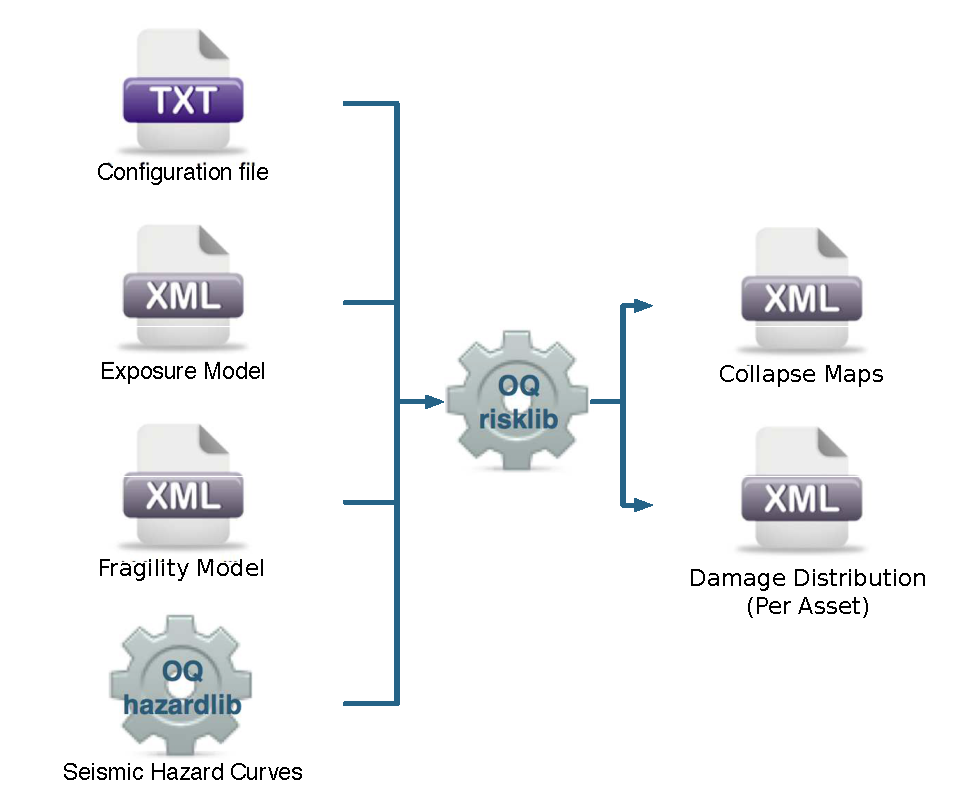
\includegraphics[width=9cm,height=7cm]{figures/risk/io-structure-classical-damage.pdf}
\caption{Classical PSHA-based Damage Calculator input/output structure.}
\label{fig:io-structure-classical-damage}
\end{figure}